\documentclass[xcolor=dvipsnames]{beamer}
\usepackage[T1]{fontenc}
\usepackage[utf8]{inputenc}
\usepackage[english,slovak]{babel}

\usepackage{amsmath}
\usepackage{amsthm}
\usetheme{Pittsburgh}
\useoutertheme{shadow}

\usepackage{graphicx}
\usepackage{caption}
\usepackage{subcaption}

\usepackage[]{algorithm2e}
\usepackage{listings}
 \setbeamercovered{transparent}
 \usepackage{cuted}
\usepackage[export]{adjustbox}
\usepackage{mathtools}

\usepackage{lipsum}

\newcommand\Wider[2][3em]{%
\makebox[\linewidth][c]{%
  \begin{minipage}{\dimexpr\textwidth+#1\relax}
  \raggedright#2
  \end{minipage}%
  }%
}

%-------------------------------------------------------------------------------------
\title{\bf Reinforcement learning}
\author{Michal CHOVANEC, PhD.}


%\setbeamertemplate{footline}[frame number]{}
\setbeamertemplate{navigation symbols}{}


\date[EURP]{\it March 2018}
\begin{document}

\begin{frame}
\titlepage
\centering{Fakulta riadenia a informatiky}
\end{frame}


\begin{frame}{\bf Problem definition}
\begin{itemize}
 \item learn to play game with unknow rules
 \item input  : state and reward
 \item output : action and total score
\end{itemize}
\centering

{\bf Agent never see required value (required action)}


\begin{figure}
\centering
\begin{minipage}{.5\textwidth}
  \centering
  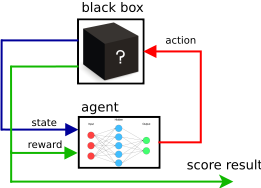
\includegraphics[scale=0.2]{../../diagrams/rl_mechanism.jpg}
\end{minipage}%
\begin{minipage}{.5\textwidth}
  \centering
  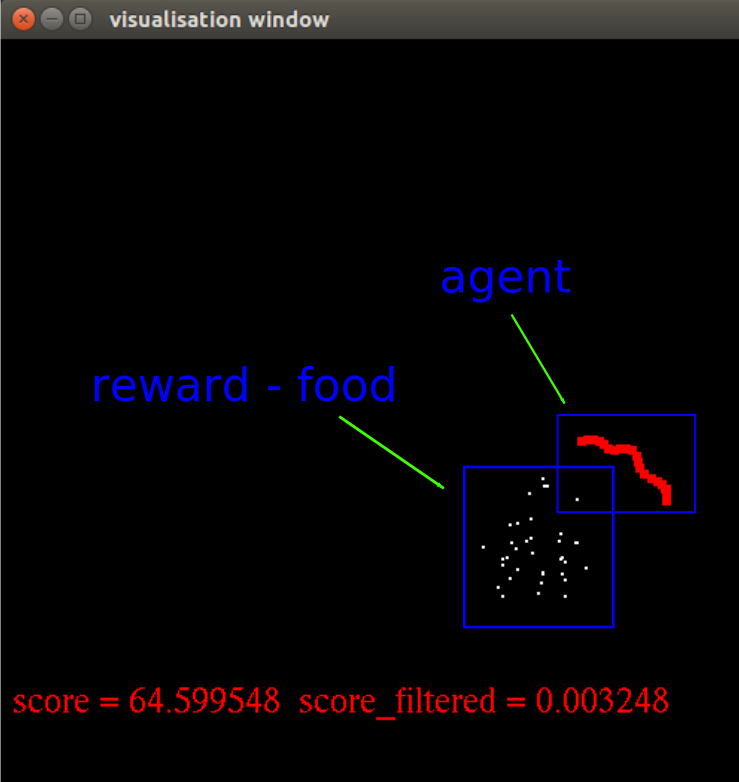
\includegraphics[scale=0.2]{../../diagrams/worms_rl_game_desc.png}
\end{minipage}
\end{figure}



\end{frame}


\begin{frame}{\bf Q-learning algorithm}
\begin{align*}
Q'(s, a) = R(s, a) + \gamma \max_{a' \in A}Q(s', a')
\end{align*}
where \\
$Q(s, a)$ is previous state \\
$Q(s', a')$ is actual state \\
$R(s, a)$ is reward obtained in state $s$ after executing action $a$ \\
$\gamma$ is discount factor $\gamma \in \langle0, 1\rangle$ \\
\begin{figure}[htbp]
  \centering
  \includegraphics[scale=0.3]{../../diagrams/q_learning_detail.jpg}
\end{figure}



\end{frame}


\begin{frame}{\bf SARSA algorithm}
State Action Reward State Action
\begin{align*}
Q'(s, a) = (1-\alpha)Q(s, a) + \alpha(R(s, a) + \gamma Q(s', a'))
\end{align*}
where \\
$Q(s, a)$ is previous state \\
$Q(s', a')$ is actual state \\
$R(s, a)$ is reward obtained in state $s$ after executing action $a$ \\
$\gamma$ is discount factor $\gamma \in \langle0, 1\rangle$ \\
$\alpha$ is learning rate $\alpha \in (0, 1)$
\begin{figure}[htbp]
  \centering
  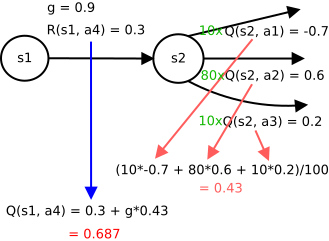
\includegraphics[scale=0.17]{../../diagrams/sarsa_learning_detail.png}
\end{figure}


\end{frame}


\begin{frame}{\bf Storing Q values}

\begin{itemize}
 \item table
 \item linear combination of basis function (handmade features)
 \item Kenerva's sparse encoding
 \item neural network
\end{itemize}

problems
\begin{itemize}
 \item state correlations
 \item nonstationary Q values
 \item convergence to optimal strategy
\end{itemize}

\end{frame}


\begin{frame}{\bf Neural network example - deep reinforcement learning}

\begin{figure}[htbp]
  \centering
  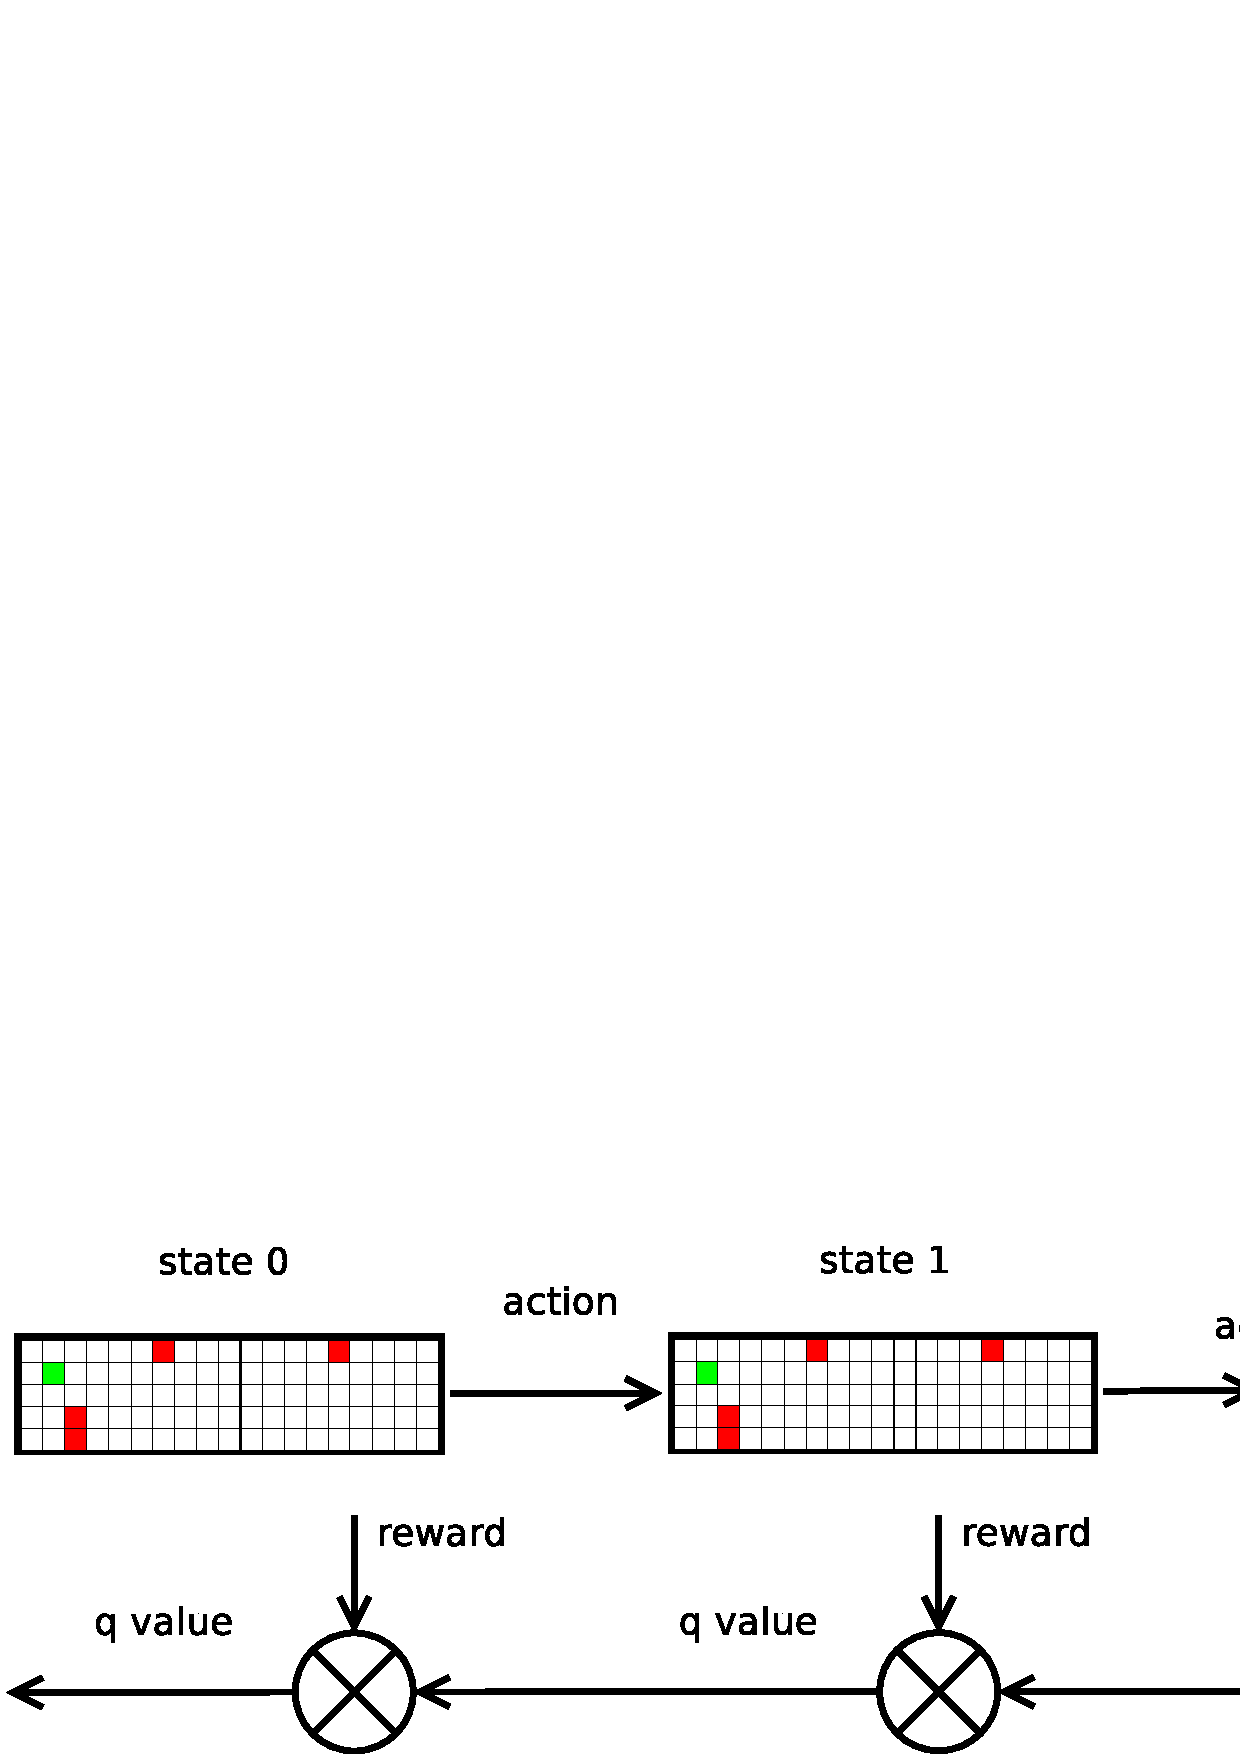
\includegraphics[scale=0.3]{../../diagrams/rl_nn_learn.png}
\end{figure}


\begin{figure}[htbp]
  \centering
  \includegraphics[scale=0.3]{../../diagrams/fnn.png}
\end{figure}

\end{frame}

%-------------------------------------------------------------------------------------
\begin{frame}{\bf Q\&A}

\begin{figure}[ht]
\begin{center}
\begin{minipage}{0.8\linewidth}
\begin{center}
 \includegraphics[width=1.0\textwidth]{../../pictures/me.jpg}
\end{center}
\end{minipage}
\end{center}
\end{figure}

\url{https://github.com/michalnand/robotics}
\url{https://github.com/michalnand/machine\_learning}

\centerline{michal.nand@gmail.com}

\end{frame}

\end{document}
